\subsection{研究背景}
%\section{Problem}
%\subsection{Background}
\setfoot{.5}
\begin{frame}{业务过程与事件日志}
	\begin{itemize}
	\item 业务过程
		\begin{itemize}
			\item [-]为达特定业务目标,按网状结构组织的一组的任务。
			\item [-]一次运行产生一条轨迹(任务执行序列)。
		\end{itemize}
	\item 事件日志
		\begin{itemize}
			\item [-]对业务过程运行的记录,由多个轨迹组成的包(bag)。
		\end{itemize}
	\item 噪声的存在
		\begin{itemize}
			\item [-]导致轨迹跟业务过程真实运行情况不符。
		\end{itemize}
	\end{itemize}
\begin{figure}
 \begin{center}
 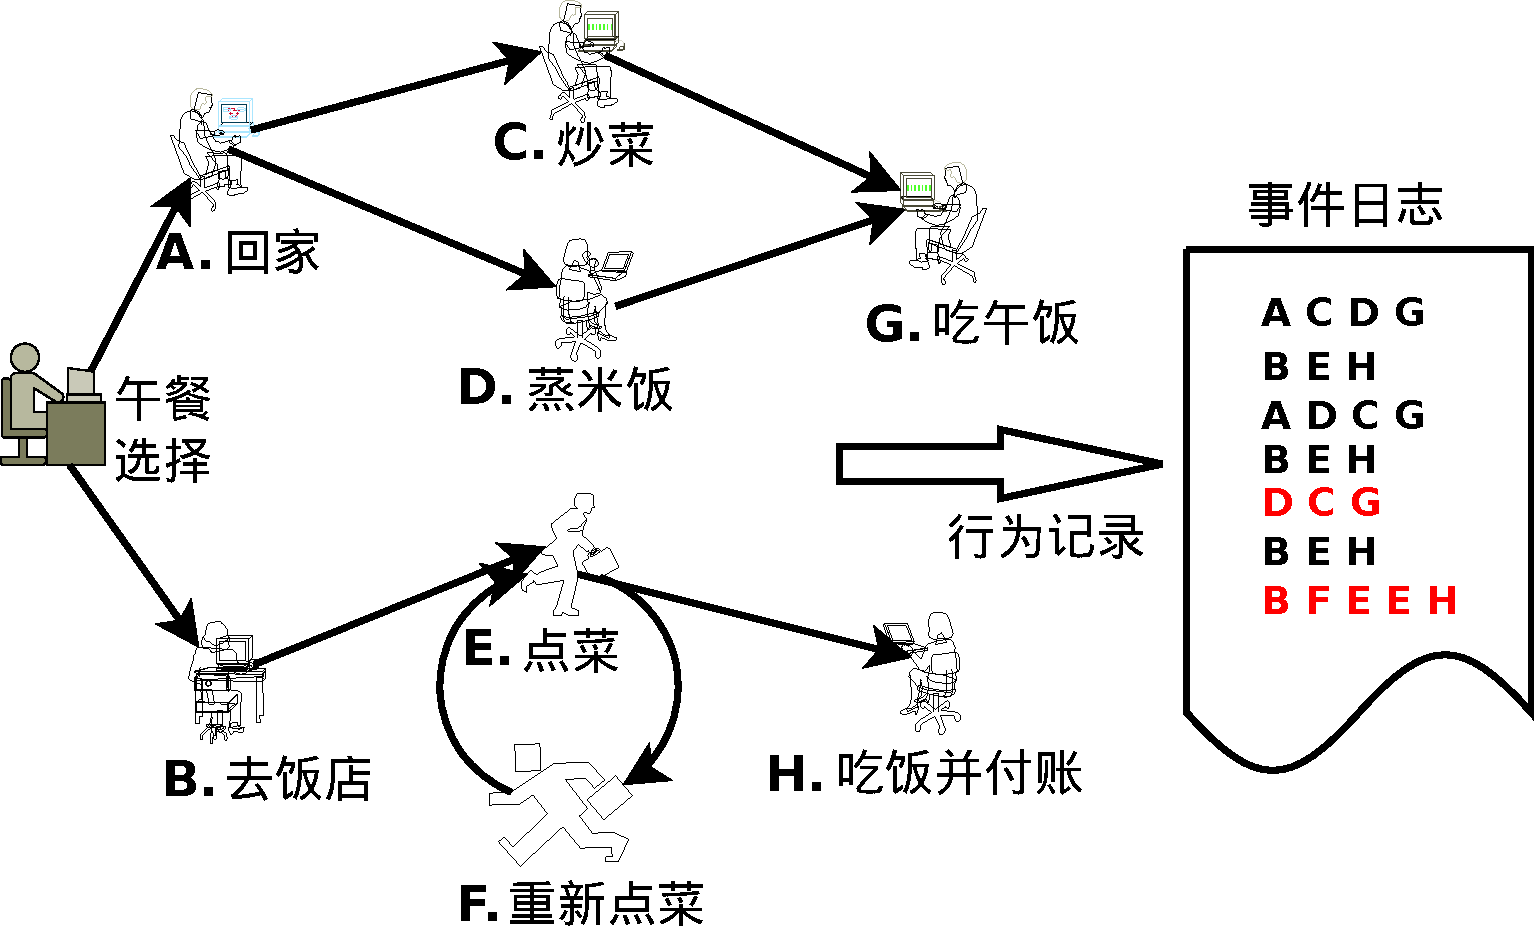
\includegraphics[width=0.7\textwidth]{lunchlog}
 \end{center}
\end{figure}
\note{业务过程与轨迹是业务过程管理领域的核心概概念。
	如图所示,一个业务过程就是一个由相互依赖的任务构成的网络,
	业务过程的一次执行产生一个轨迹,一条轨迹简单说就是一个由任务名称组成的字符串,
	多条轨迹记录下来就是日志。
%	说明业务过程是一个任务网络,业务过程执行一次就产生一轨迹,轨迹就是一个任务序列。
%日志是由轨迹组成的包,包中同一条轨迹可以出现多次。因为噪声的存在,导致轨迹跟真实发现的任务
%序列不一致,即产生污损轨迹。\\
%吃午饭这个例子,包含两个场景,回家自己做着吃,与吃饭店;回家吃饭,首先要回家,然后可以并行地蒸米饭与炒菜,最后吃饭;吃饭店则首先要去饭店,然后点菜,如果点的菜没有了,要重新点菜,最后吃饭付款。\\
%每次午饭,都有一条轨迹记录,如右边
%的日志,由于噪声,有些轨迹受到污损,如红色轨迹所示,回家的任务漏记了;以及点菜与再次点任务颠倒了\\
0.5分钟}
\end{frame}
%\begin{frame}{业务过程管理(Business Process Management,BPM)}
%	\begin{itemize}
%	\item 业务过程管理为业务过程及相关资源的设计、部署与分析等提供方法、技术、软件等工具。
%	\item 业务过程管理的实施,一般都有离不开某种过程感知的信息系统(PAIS)的支撑
%	\item 过程挖掘是BPM中一项重要研究课题。
%	\end{itemize}
%\begin{figure}
% \begin{center}
% \includegraphics[width=0.8\textwidth]{bpmlifecycle}
% \end{center}
%\end{figure}
%\end{frame}
\setfoot{1控制流}
\begin{frame}{过程挖掘}
	\begin{itemize}
	\item 基于业务过程运行的真实情况记录(日志)挖掘相关的知识
	\item 在实施过程中,过程建模占用$60\%\sim 80\%$的时间\tfn{J. Herbst, D. Karagiannis. Integrating Machine Learning and Workflow Management to
 Support Acquisition and Adaptation of Workflow Models. International Journal of Intelligent
  Systems in Accounting, Finance and Management, 2000, 9:67–92}。%\cite{herbstacc}
	\end{itemize}
\begin{figure}
 \begin{center}
 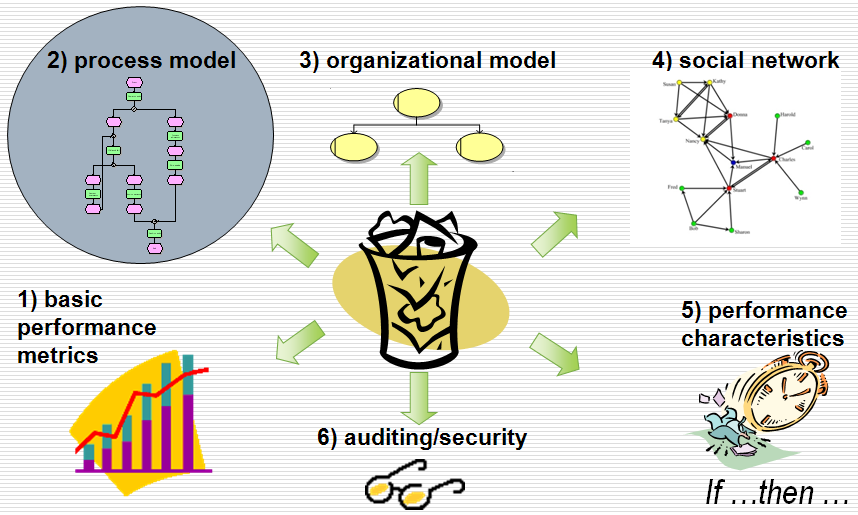
\includegraphics[width=0.9\textwidth]{pmfunctions}
 \end{center}
\end{figure}
\note{过程挖掘是业务过程领域的研究热点。
	所谓过程挖掘,就是从事件日志中挖掘有用的知识。
	包括挖掘性能因素、控制流挖掘、组织架构等等。
	由于具体的实施过程中,过程建模占用太多的时间,所以我们重点关注过程控制流的挖掘。
	%在点明过程挖掘是从日志中挖掘知识,读出其六大功能,说明建模比较费劲,强调我们关注控制流挖掘。\\
0.5分钟}
\end{frame}
\setfoot{1.5}
\begin{frame}{控制流挖掘}
	\begin{itemize}
	\item 从事件日志数据中,挖掘出一个合理的业务过程模型。
	\end{itemize}
\begin{figure}
 \begin{center}
 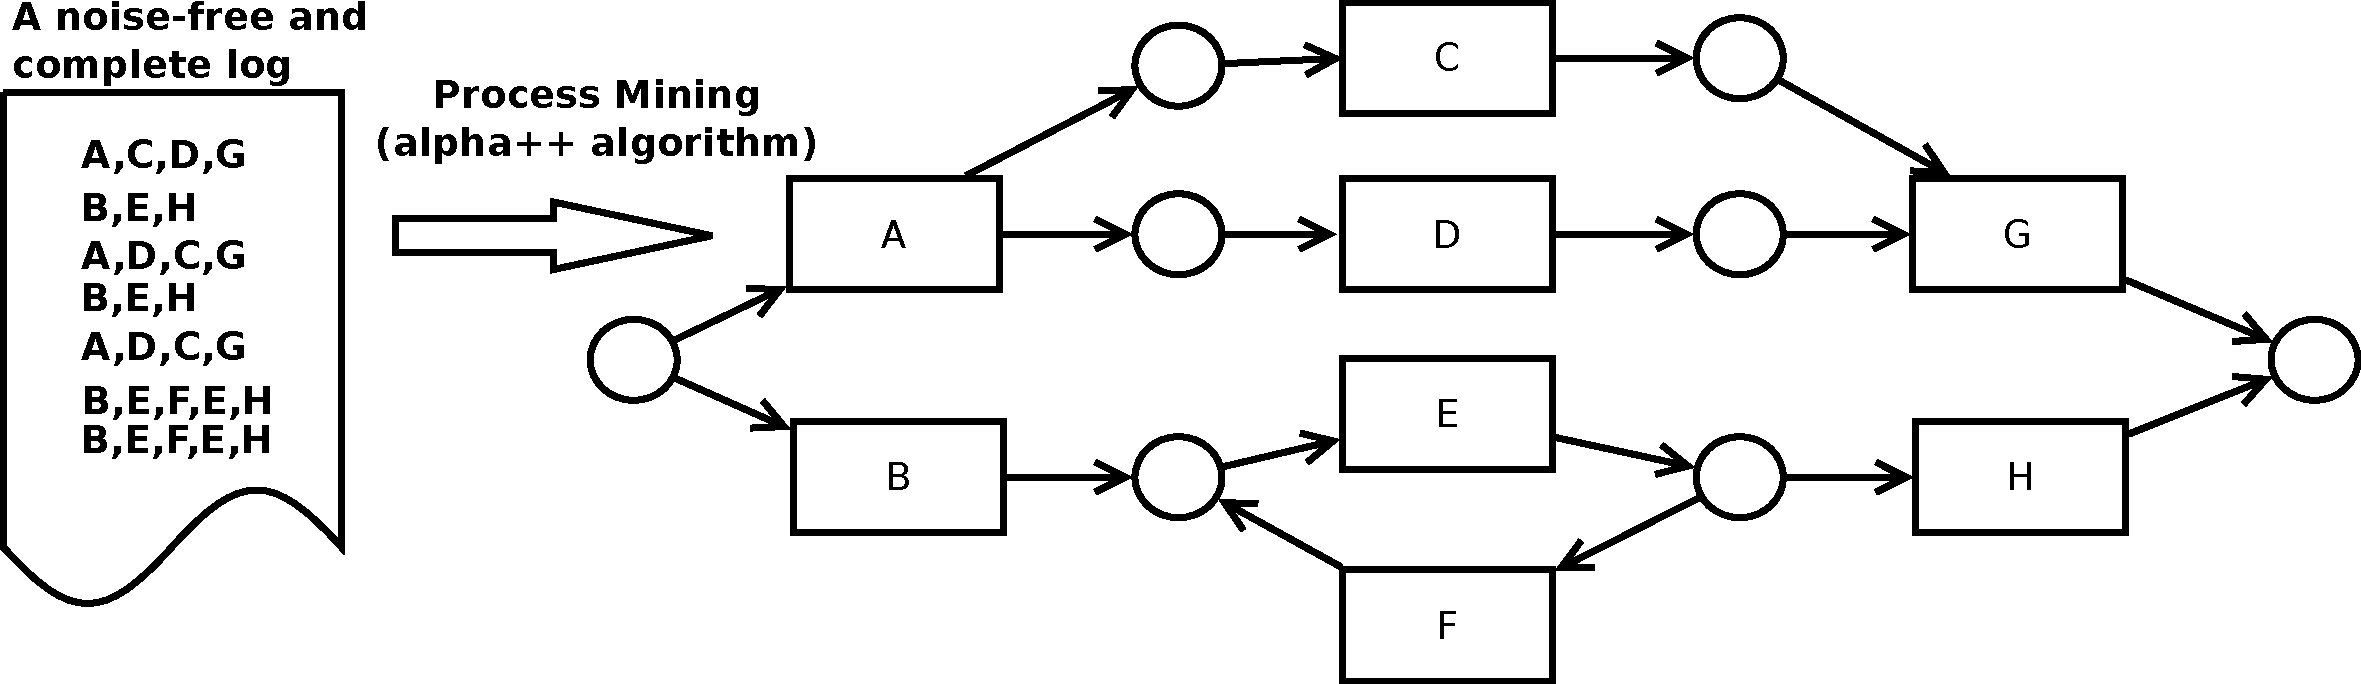
\includegraphics[width=1.0\textwidth]{processmining}
 \end{center}
\end{figure}
\begin{itemize}
	\item 挖掘结果质量依赖于
		\begin{itemize}
			\item 所用算法
			\item 数据(日志)质量
		\end{itemize}
\end{itemize}
\note{如图所示,所谓控制流挖掘就是从日志中挖掘出合理的流程模型。
	%强调模型挖掘要挖掘出合理的过程模型,或者说是任务有向图的结构信息,此处日志是前面所示吃午饭的事件日志,强调它未受噪声影响且局部信息完备,利用alpha++算法可以准确地得到午饭过程的控制模型。
	一般说来,挖掘结果的质量,一方向受限于挖掘算法的能力,另一方面取决于日志数据的质量。\\
0.5分钟}
\end{frame}

